% Arquivo principal para o Overleaf. Compilador: pdfLaTeX.
% Artigo completo; preencher apenas os dados reais de autoria antes da entrega.
% Formatação extraída do template COTB 2027 fornecido.
% Compatibilidade: language=english por último mantém inglês como padrão
% do babel, sem a chave aninhada main=english que falha em xkeyval antigo.
\documentclass[sigconf, nonacm, screen, language=portuguese, language=spanish, language=english]{acmart}             % VERSAO FINAL

\AtBeginDocument{%
  \providecommand\BibTeX{{%
    \normalfont B\kern-0.5em{\scshape i\kern-0.25em b}\kern-0.8em\TeX}}}

%% NAO carregue o pacote babel manualmente: a classe acmart ja o
%% carrega automaticamente com os idiomas indicados nas opcoes
%% "language=..." do \documentclass acima (evita conflito de dupla
%% carga do babel).
\usepackage{amsmath}
\usepackage{amsfonts}
\let\Bbbk\relax
\usepackage{amssymb}
\usepackage{booktabs}
\usepackage{multirow}
\usepackage{graphicx}

%% Remove o bloco de identificacao ACM (nao se aplica ao evento)
\settopmatter{printccs=false, printacmref=false}
\renewcommand\footnotetextcopyrightpermission[1]{}

%% =====================================================================
%% CABECALHO PERSONALIZADO (dados do evento a esquerda, autores a
%% direita)
%% ---------------------------------------------------------------------
%% - O lado ESQUERDO do cabecalho traz o nome/edicao do evento, local
%%   e datas. Edite a macro \cotbEventInfo abaixo se necessario.
%% - O lado DIREITO do cabecalho traz os autores do trabalho:
%%     * ate 3 (tres) autores: lista todos os nomes (gerado
%%       automaticamente a partir dos comandos \author usados mais
%%       abaixo, no mesmo formato usado pela classe acmart);
%%     * mais de 3 (tres) autores: exibe apenas o PRIMEIRO autor
%%       seguido de "et al." (tambem gerado automaticamente).
%%   Nao e necessario editar nada manualmente: o comportamento eh
%%   determinado pela quantidade de comandos \author preenchidos
%%   na secao de autores, logo abaixo.
%% =====================================================================
\makeatletter
\newcounter{cotbNumAuthors}
\let\cotb@originalauthor\author
\renewcommand{\author}[1]{%
  \stepcounter{cotbNumAuthors}%
  \ifnum\value{cotbNumAuthors}=1
    \gdef\cotbFirstAuthorName{#1}%
  \fi
  \cotb@originalauthor{#1}%
}
\makeatother

%% Dados do evento exibidos do lado esquerdo do cabecalho (mantenha
%% o texto curto, em ate duas linhas, para nao colidir com o lado
%% direito):
\newcommand{\cotbEventInfo}{XVIII Computer on the Beach (COTB 2027)\\
  Florianópolis/SC --- 13 a 17 de abril de 2027}

%% Autores exibidos do lado direito do cabecalho (logica automatica
%% de "et al." para mais de 3 autores):
\newcommand{\cotbHeaderAuthors}{%
  \ifnum\value{cotbNumAuthors}>3
    \cotbFirstAuthorName\ et al.%
  \else
    \shortauthors
  \fi
}

%% Espaco reservado para o cabecalho de duas linhas nao colidir com
%% o corpo do texto:
\setlength{\headheight}{24pt}

\AtBeginDocument{%
  \fancypagestyle{firstpagestyle}{%
    \fancyhf{}%
    \renewcommand{\headrulewidth}{0.4pt}%
    \renewcommand{\footrulewidth}{0pt}%
    \fancyhead[L]{\begin{minipage}[b]{0.62\textwidth}\raggedright
      \scriptsize\cotbEventInfo\end{minipage}}%
    \fancyhead[R]{\begin{minipage}[b]{0.34\textwidth}\raggedleft
      \scriptsize\cotbHeaderAuthors\end{minipage}}%
    \fancyfoot[C]{\if@ACM@printfolios\thepage\fi}%
  }%
  \fancypagestyle{standardpagestyle}{%
    \fancyhf{}%
    \renewcommand{\headrulewidth}{0.4pt}%
    \renewcommand{\footrulewidth}{0pt}%
    \fancyhead[L]{\begin{minipage}[b]{0.62\textwidth}\raggedright
      \scriptsize\cotbEventInfo\end{minipage}}%
    \fancyhead[R]{\begin{minipage}[b]{0.34\textwidth}\raggedleft
      \scriptsize\cotbHeaderAuthors\end{minipage}}%
    \fancyfoot[C]{\if@ACM@printfolios\thepage\fi}%
  }%
  %% IMPORTANTE: a classe acmart ja executa "\pagestyle{standardpagestyle}"
  %% durante o carregamento (antes desta redefinicao ter efeito). Por
  %% isso, e necessario chamar \pagestyle novamente aqui, para que o
  %% cabecalho das paginas internas passe a usar a versao customizada
  %% definida acima (evento a esquerda, autores a direita).
  \pagestyle{standardpagestyle}%
}

\usepackage{tabularx}
% Gerado das evidências de execução; não editar valores manualmente.
\newcommand{\UnitTests}{36}
\newcommand{\InstrumentedTests}{6}
\newcommand{\UnitSeconds}{5,36}
\newcommand{\StartupMedian}{3095}
\newcommand{\StartupMin}{2886}
\newcommand{\StartupMax}{3714}
\newcommand{\FavoriteMedian}{10,35}
\newcommand{\MemoryPss}{123,69}


\begin{document}

\title{Software Architecture Analysis of Now in Android}
\translatedtitle{portuguese}{Análise da Arquitetura de Software do Now in Android}

% Preencher um bloco por autor. Não inferir autoria a partir do computador.
\author{[Nome completo do autor]}
\affiliation{%
  \institution{[Instituição]}
  \streetaddress{[Endereço]}
  \city{[Cidade]}
  \state{[Estado]}
  \country{Brasil}}
% Descomentar após preencher o endereço real:
% \email{nome@instituicao.br}

\begin{abstract}
This paper examines the software architecture of Now in Android through
static inspection of a fixed repository revision, its architecture guides,
modules, data flows, tests, and build workflow. The study relates stakeholder
concerns to architectural views and a Goal/Question/Metric evaluation plan.
The inspected code combines a layered structure, ViewModels, unidirectional
data flow, repositories, dependency injection, and local storage with
synchronization. An outdated use-case example in the architecture guide is
distinguished from the current implementation. A separate four-module Android
application demonstrates a local news catalog and persistent bookmarks using
Compose, Flow, Hilt, and Room. The evaluation approved 36 unit tests and six instrumented tests
in the evaluated environment. Structural checks and exploratory runtime
measurements characterize the demonstration without establishing causal
improvements or measuring the original application. Task completion and task
time with actual users remain proposed evaluations. The contribution is a
traceable connection between the inspected architecture, a smaller working
implementation, and explicit limits on quality claims.
\end{abstract}

\keywords{Software architecture, Android, Now in Android, Modularization,
Goal Question Metric}

\maketitle
\selectlanguage{portuguese}

\section{Introdução}\label{sec:introducao}
Decisões arquiteturais organizam responsabilidades e dependências e afetam
como equipes desenvolvem e verificam um sistema. Entretanto, reconhecer um
padrão no código não demonstra, por si só, melhoria de qualidade. É necessário
relacionar a decisão a interesses, perguntas e evidências.

Este trabalho analisa o Now in Android (NiA), projeto aberto do Google que
serve de referência para desenvolvimento Android~\cite{nowinandroid,android-arquitetura}. O
objetivo é identificar suas decisões arquiteturais e aplicá-las, com
simplificações justificadas, a uma demonstração de notícias e favoritos.
O método consiste em inspeção estática de uma revisão fixada, análise dos
stakeholders, construção de vistas e de um plano Goal/Question/Metric
(GQM), seguida de implementação e testes de um aplicativo independente.
As medições executadas pertencem exclusivamente à demonstração.

A Seção~\ref{sec:fundamentacao} apresenta os conceitos utilizados e a
Seção~\ref{sec:metodos}, o método. As Seções~\ref{sec:projeto} a
\ref{sec:diagramas} caracterizam o NiA e analisam stakeholders, vistas,
qualidade e arquitetura. A Seção~\ref{sec:projeto-base} descreve a
demonstração e seus resultados, discutidos na Seção~\ref{sec:discussao}; a
Seção~\ref{sec:conclusao} conclui o trabalho.

\begin{figure*}[t]
\centering
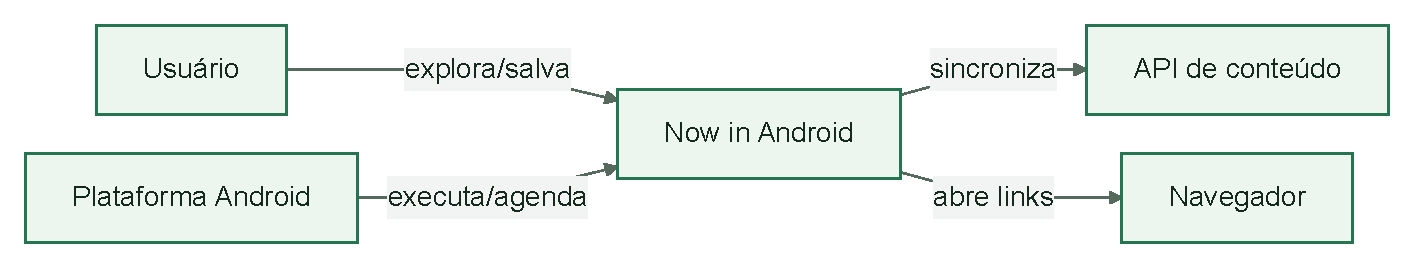
\includegraphics[width=\textwidth]{imagens/01-contexto.pdf}
\caption{Contexto do NiA: interação do leitor, conteúdo remoto, navegação
externa e serviços da plataforma. Armazenamentos internos são detalhados nas
outras vistas.}
\Description{O usuário explora o aplicativo; o aplicativo sincroniza com a API e abre links no navegador; a plataforma Android executa e agenda trabalho.}
\label{fig:contexto}
\end{figure*}

\section{Caracterização do Projeto Estudado}\label{sec:projeto}
O NiA apresenta conteúdos da série Now in Android e permite acompanhar tópicos
e salvar recursos. Atende leitores interessados no ecossistema e
programadores que estudam suas práticas. O recorte usa o commit
\texttt{2982e63}, de 20/10/2026; o hash completo, os arquivos consultados e os
links permanentes estão no relatório complementar. A coleta foi realizada
em 15/11/2026. A Tabela~\ref{tab:caracterizacao} resume a elegibilidade.

\begin{table}[htb]
\caption{Caracterização e evidências do NiA na revisão estudada.}
\label{tab:caracterizacao}
\centering
\begin{tabularx}{\columnwidth}{@{}lX@{}}
\toprule
Aspecto & Evidência \\
\midrule
Licença & Apache 2.0 \\
Tecnologias & Kotlin, Compose, Flow, Hilt, Room, DataStore e WorkManager \\
Contribuições & 1.407 PRs, abertas e encerradas, na consulta à API GitHub \\
Atividade & PR \#2142 integrada em 20/10/2026 \\
Testes recentes & \texttt{For\allowbreak You\allowbreak View\allowbreak Model\allowbreak Test} alterado em 16/10/2026 \\
Automação & Workflow \texttt{Build.yaml}: testes, APKs, screenshots e lint \\
\bottomrule
\end{tabularx}
\end{table}

A existência desses artefatos atende ao recorte exigido de atividade e testes
recentes, mas não significa que a suíte original tenha sido executada neste
estudo. A Figura~\ref{fig:contexto} delimita o contexto operacional.

\begin{figure*}[t]
\centering
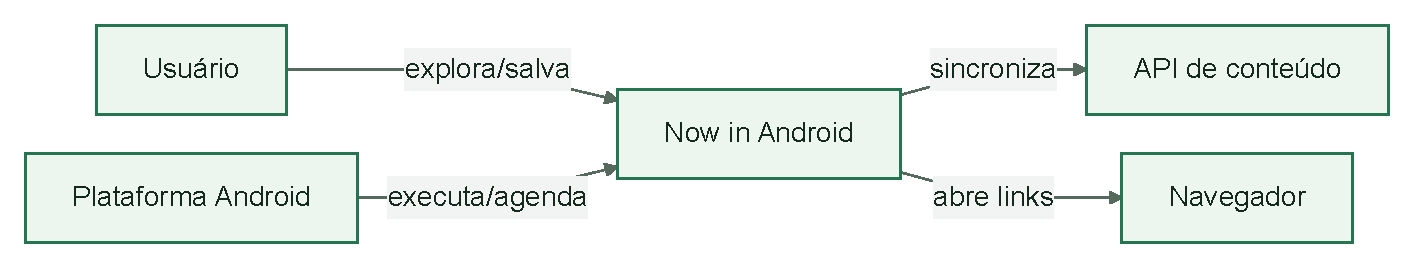
\includegraphics[width=\textwidth]{imagens/01-contexto.pdf}
\caption{Contexto do NiA: interação do leitor, conteúdo remoto, navegação
externa e serviços da plataforma. Armazenamentos internos são detalhados nas
outras vistas.}
\Description{O usuário explora o aplicativo; o aplicativo sincroniza com a API e abre links no navegador; a plataforma Android executa e agenda trabalho.}
\label{fig:contexto}
\end{figure*}

\section{Análise dos Stakeholders}\label{sec:stakeholders}
A Tabela~\ref{tab:stakeholders} organiza seis papéis. As funcionalidades,
contribuições e testes sustentam sua identificação; necessidades e conflitos
são inferências analíticas, sem entrevistas. Não se afirma a existência de
seis equipes separadas na organização do projeto.

\begin{table*}[t]
\caption{Stakeholders: evidência do papel e necessidades inferidas.}
\label{tab:stakeholders}
\centering
\begin{tabularx}{\textwidth}{@{}lXX@{}}
\toprule
Parte interessada & Evidência observada & Interesse e necessidade inferidos \\
\midrule
Usuários & Leitura, tópicos e recursos salvos & Conteúdo pertinente, navegação clara e acesso local \\
Desenvolvedores & Módulos, código e PRs & Compreender limites, implementar mudanças e testar isoladamente \\
Mantenedores & Revisões, documentação e automação & Conservar coerência, estabilidade e builds viáveis \\
Produtores de conteúdo & Série NiA referenciada pelo aplicativo & Conteúdo correto e atualizado; processo editorial não auditado \\
Qualidade & Testes JVM, instrumentados e screenshots & Reproduzir falhas e verificar estados e persistência \\
Plataforma Android & APIs Jetpack e objetivo de referência & Evoluir práticas e manter exemplos compreensíveis \\
\bottomrule
\end{tabularx}
\end{table*}

\begin{table}[htb]
\caption{Conflitos possíveis e encaminhamentos propostos.}
\label{tab:conflitos}
\centering
\begin{tabularx}{\columnwidth}{@{}XX@{}}
\toprule
Interesses em tensão & Encaminhamento \\
\midrule
Atualização do conteúdo versus rede e bateria & Leitura local e trabalho de sincronização agendado \\
Novas APIs versus estabilidade e compreensão & Versões fixadas, revisão e testes de regressão \\
Isolamento das features versus custo de configuração & Módulos proporcionais ao escopo e regras de dependência \\
\bottomrule
\end{tabularx}
\end{table}

Esses conflitos não são incidentes comprovados. São hipóteses úteis para
justificar critérios de avaliação e explicitar os custos das decisões.

\section{Pontos de Vista Arquiteturais}\label{sec:vistas}
\textbf{Usuário.} A seleção de tópicos personaliza o feed; favoritos permitem
reencontrar recursos. A leitura local mantém conteúdo já persistido quando
não há rede, mas não assegura atualização nem acesso aos links externos.
A navegação e os estados de interface tornam essas funções observáveis.

\textbf{Desenvolvimento.} O módulo aplicativo reúne inicialização e navegação;
features separam funcionalidades; componentes \texttt{core} compartilham dados,
modelos e UI. Interfaces de repositórios e dependências explícitas apoiam
substituição em testes. No original, features como For You usam módulos
\texttt{api}/\texttt{impl}~\cite{nia-modularizacao}.

\textbf{Operação e manutenção.} A sincronização conecta rede e persistência.
O trabalho é coordenado pelo \texttt{Sync\allowbreak Worker}, que permite novas tentativas.
O workflow inspecionado declara testes, build e lint. Ele evidencia mecanismos
de verificação, sem provar ausência de falhas ou uma taxa histórica de sucesso.

\section{Atributos de Qualidade com GQM}\label{sec:gqm}
O GQM deriva medidas de objetivos e perguntas, exigindo interpretação no
contexto de avaliação~\cite{basili1994}. A Tabela~\ref{tab:gqm} apresenta quatro
objetivos e três perguntas por atributo. Para o NiA, trata-se de um plano
apoiado na inspeção; a coleta técnica foi aplicada ao aplicativo demonstrativo.

\begin{table*}[t]
\caption{Plano GQM. M: manutenibilidade; T: testabilidade; D: desempenho;
U: usabilidade. Medidas de tarefas com pessoas permanecem propostas.}
\label{tab:gqm}
\centering
\begin{tabularx}{\textwidth}{@{}lXXX@{}}
\toprule
Objetivo & Pergunta & Métrica/unidade & Estratégia de avaliação \\
\midrule
M: separar responsabilidades & Há ciclos entre módulos? & Quantidade de ciclos & Extrair e percorrer o grafo Gradle \\
M & Há dependências entre features? & Arestas feature--feature & Filtrar dependências diretas \\
M & A UI conhece a persistência? & Referências indevidas & Buscar tipos de Room/DAO nas features e UI \\
T: verificar com isolamento & Classes aceitam substitutos? & Classes testadas com fakes & Inspecionar casos e dependências dos testes \\
T & Os casos previstos passam? & Aprovados/executados & Consolidar relatórios JUnit \\
T & Quanto custa executar a suíte? & Tempo de parede (s) & Cronometrar a chamada de testes unitários \\
D: caracterizar execução & Quanto leva iniciar a Activity? & Mediana e intervalo (ms) & Dez reinícios do processo; \texttt{am start -W} \\
D & Quanto leva atualizar o fluxo? & Latência de emissão (ms) & Dez gravações alternadas com coletor ativo \\
D & Qual o uso após o roteiro? & PSS (MiB) & Uma captura \texttt{dumpsys meminfo} \\
U: avaliar clareza das ações & Controles têm rótulo e área? & Aprovados/5; mínimo 48 dp & Inspeção automatizada de cinco controles \\
U & Leitores concluem as tarefas? & Conclusões/tentativas (\%) & Sessões com pessoas: avaliação proposta \\
U & Quanto demoram nas tarefas? & Tempo por tarefa (s) & Cronometragem: avaliação proposta \\
\bottomrule
\end{tabularx}
\end{table*}

As métricas estruturais se relacionam à modularização e ao encapsulamento; as
de testes, às interfaces injetáveis; tempos e memória, à execução reativa; e
os controles, à apresentação. Nenhuma medida isolada comprova o atributo
inteiro. Sem comparação ou baseline, não se atribui causalidade à arquitetura.

\section{Análise da Arquitetura do Now in Android}\label{sec:arquitetura}
\subsection{Camadas e Padrões}
A documentação descreve UI, Domain e Data, com eventos encaminhados para
operações e dados observados por Flow~\cite{nia-arquitetura}. O domínio é
opcional nas recomendações Android: encapsula regras complexas ou
reutilizadas, e pode depender da camada de dados~\cite{android-dominio}.
A Figura~\ref{fig:camadas} distingue dependências e observação de dados.

Na UI, Compose apresenta estado e encaminha ações. O ViewModel mantém
\texttt{State\allowbreak Flow} e executa operações no seu escopo. Essa organização é
compatível com MVVM, mas MVVM descreve a apresentação, não todas as decisões
do sistema. UDF descreve a direção das interações, sem exigir ligação
bidirecional entre propriedades visuais e dados.

\begin{figure*}[t]
\centering
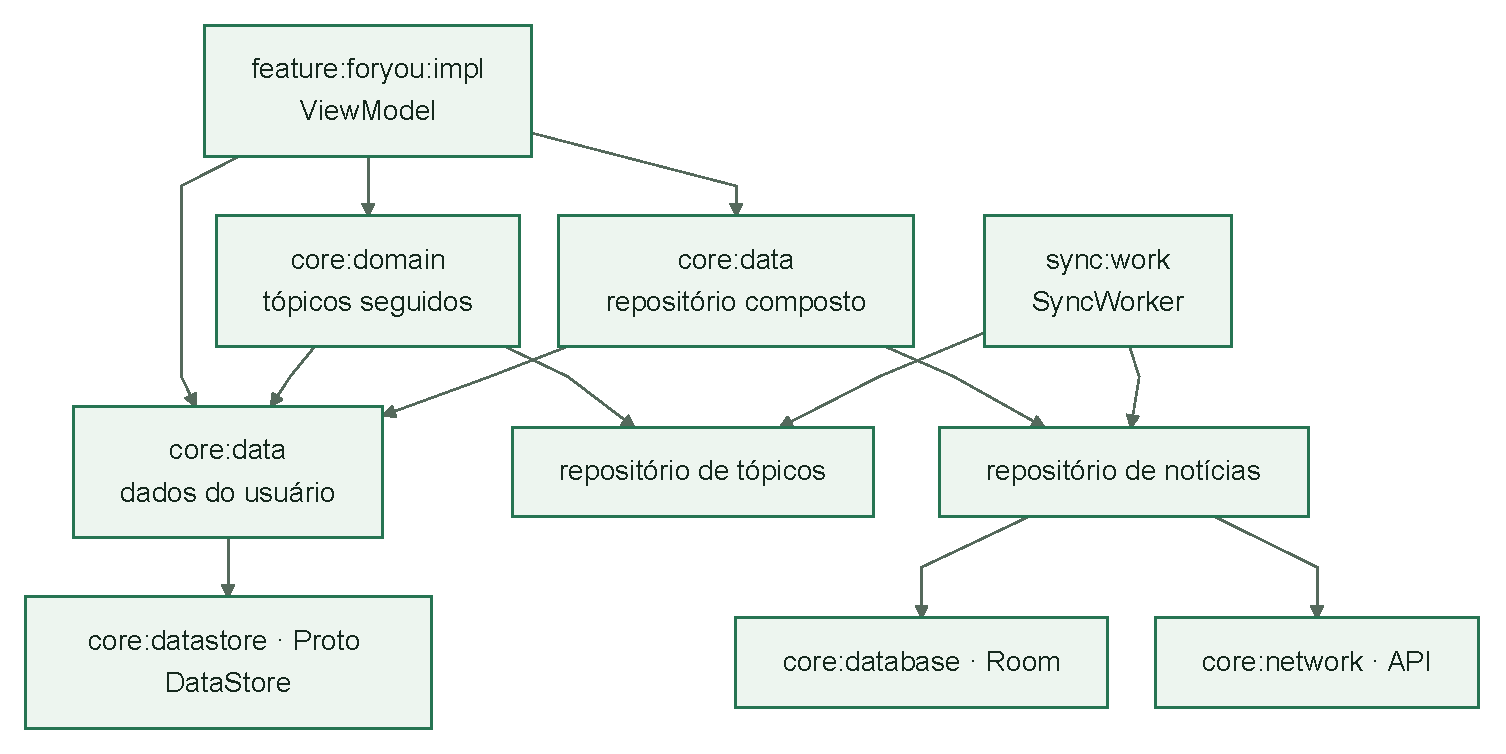
\includegraphics[width=\textwidth]{imagens/02-componentes.pdf}
\caption{Componentes do recorte For You e sincronização. Rótulos curtos
representam repositórios e módulos; não são um inventário completo do sistema.}
\Description{For You usa domínio, repositório composto e dados do usuário. O composto depende de notícias e usuário, apoiados em Room, rede e DataStore. SyncWorker coordena notícias e tópicos.}
\label{fig:componentes}
\end{figure*}

\begin{figure*}[t]
\centering
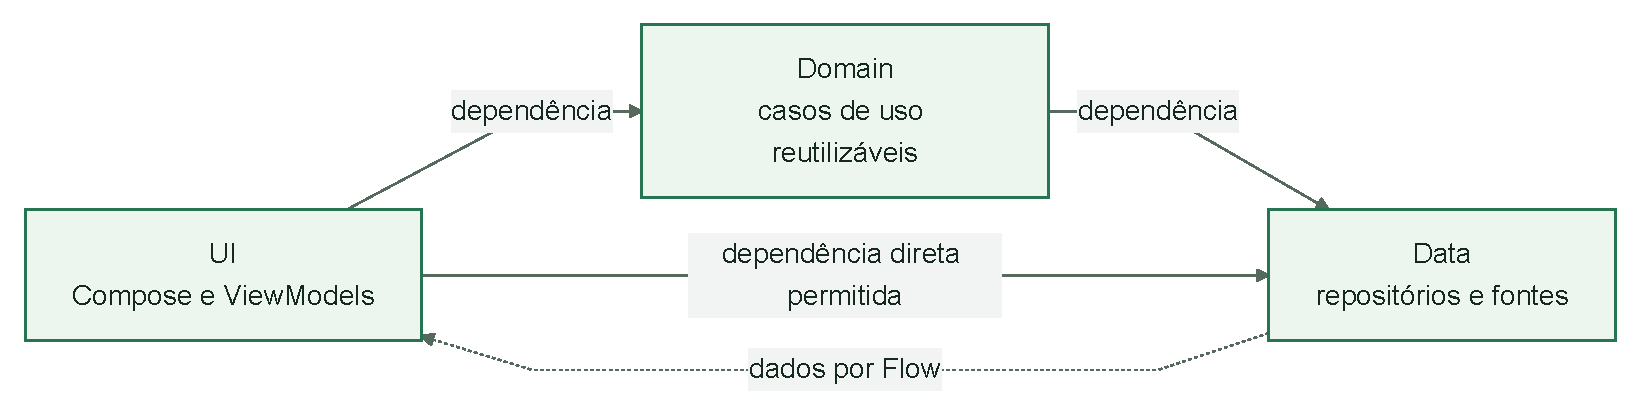
\includegraphics[width=\textwidth]{imagens/03-camadas.pdf}
\caption{Camadas do NiA. Setas contínuas indicam dependências de código;
a tracejada representa observação reativa. A UI pode usar dados diretamente.}
\Description{UI depende de Domain e Data. Domain depende de Data. Dados observáveis retornam à UI por Flow.}
\label{fig:camadas}
\end{figure*}

Na camada de dados, interfaces como \texttt{News\allowbreak Repository} e
\texttt{User\allowbreak Data\allowbreak Repository} ocultam fontes. O
\texttt{Composite\allowbreak User\allowbreak News\allowbreak Resource\allowbreak Repository} associa notícias a preferências.
Esse encapsulamento favorece substituição, mas acrescenta contratos e
coordenação de fluxos. A modularização da Figura~\ref{fig:componentes} explicita
limites; seu custo inclui configuração e evolução das dependências.

Hilt vincula interfaces a implementações em \texttt{Data\allowbreak Module} e injeta o
ViewModel; na revisão atual há também injeção assistida para a chave de
navegação. Isso reduz montagem manual, mas introduz geração de código e
configuração. O uso de Flow permite recomposição a partir de mudanças,
exigindo atenção a cancelamento, assinaturas e concorrência.

\subsection{Persistência, Sincronização e For You}
O repositório \texttt{Offline\allowbreak First\allowbreak News\allowbreak Repository} consulta Room e
sincroniza atualizações remotas.

Preferências e favoritos ficam no Proto DataStore,
acessado por \texttt{Nia\allowbreak Preferences\allowbreak Data\allowbreak Source}. WorkManager executa \texttt{Sync\allowbreak Worker}. A disponibilidade local tem como contrapartida a
possibilidade de conteúdo desatualizado e o custo de sincronização, coerente
com a orientação offline-first~\cite{android-offline}.

O feed de For You chama
\texttt{observe\allowbreak All\allowbreak For\allowbreak Followed\allowbreak Topics()} no repositório composto. Ele observa os
tópicos seguidos e combina notícias com dados do usuário; o ViewModel converte
a emissão em \texttt{News\allowbreak Feed\allowbreak Ui\allowbreak State.Success}, inicialmente \texttt{Loading}.
Para salvar, a ação \texttt{update\allowbreak News\allowbreak Resource\allowbreak Saved} delega a gravação.
O método chamado é \texttt{set\allowbreak News\allowbreak Resource\allowbreak Bookmarked}. DataStore emite a alteração e o feed é
recalculado. O domínio permanece exemplificado pelo
\texttt{Get\allowbreak Followable\allowbreak Topics\allowbreak Use\allowbreak Case}, usado no onboarding.

Há uma divergência relevante: a jornada ainda cita
\texttt{Get\allowbreak User\allowbreak News\allowbreak Resources\allowbreak Use\allowbreak Case}, ausente na árvore estudada. Por isso,
a sequência usa os participantes do código atual. A organização em camadas
não constitui evidência de adesão integral a Clean Architecture ou Arquitetura
Hexagonal; essas classificações exigiriam verificar suas regras específicas.

\section{Diagramas Arquiteturais}\label{sec:diagramas}
As Figuras~\ref{fig:contexto}--\ref{fig:demo} oferecem vistas complementares.
A Figura~\ref{fig:sequencia} detalha a leitura local e a gravação do favorito;
a sincronização remota é um fluxo complementar, não uma chamada direta do
ViewModel à rede. Os fontes Mermaid e as exportações vetoriais acompanham a
entrega para revisão das relações.

\begin{figure*}[t]
\centering
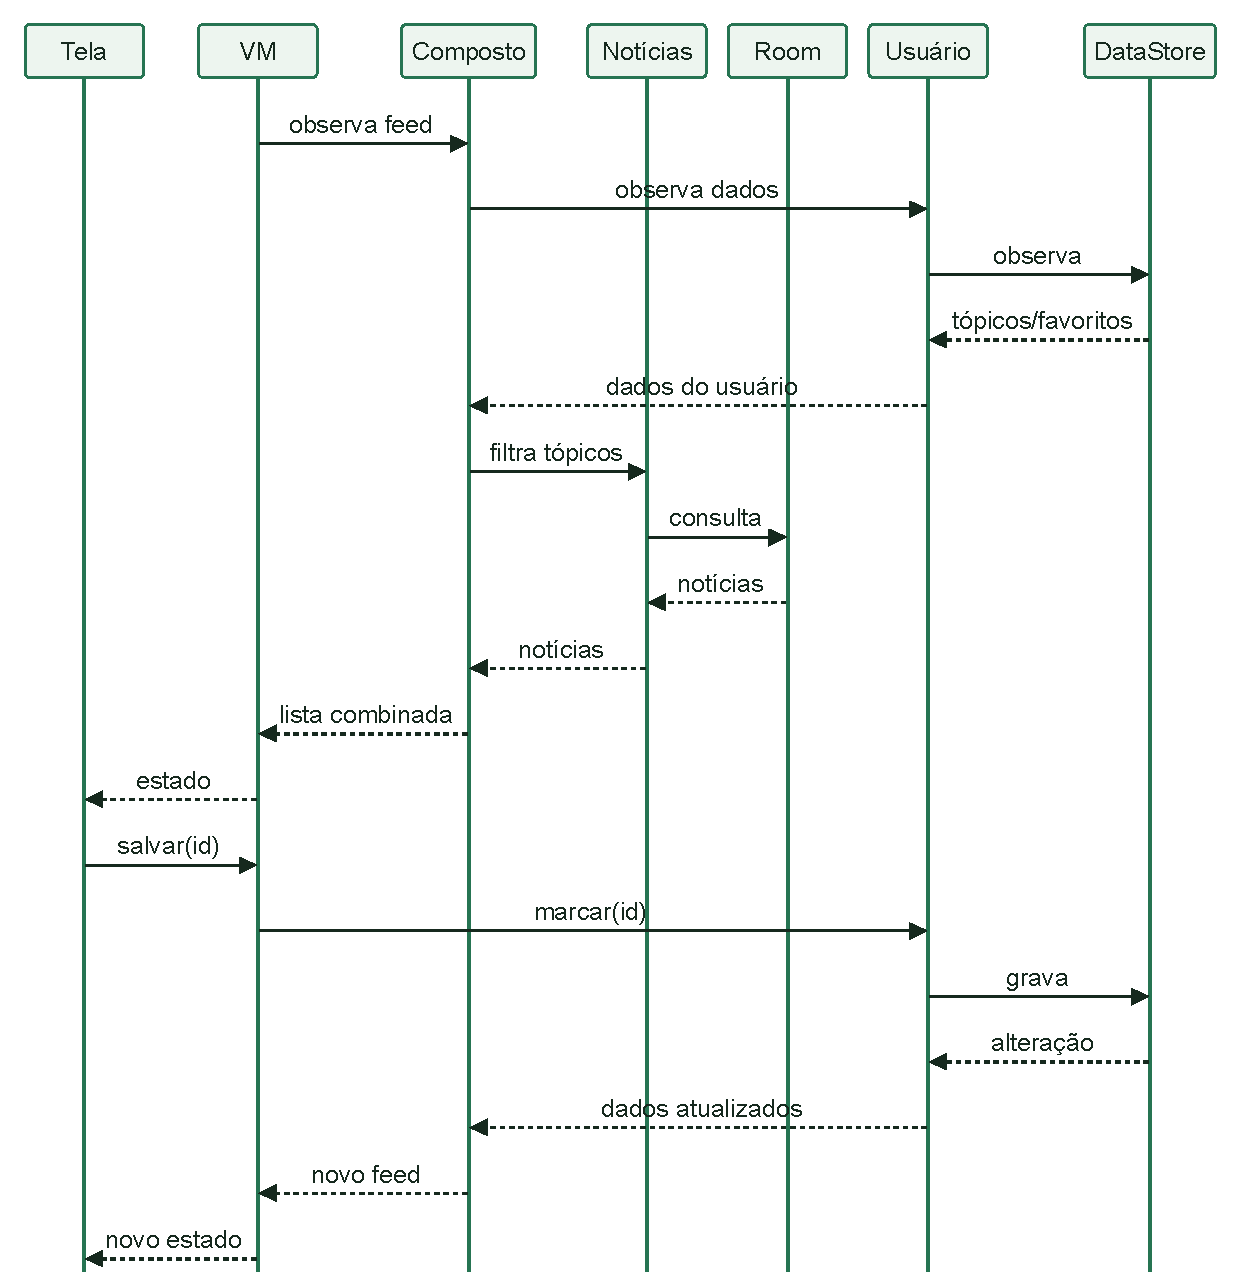
\includegraphics[width=.90\textwidth]{imagens/04-sequencia.pdf}
\caption{Sequência atual do recorte For You. ``Composto'' representa
CompositeUserNewsResourceRepository; ``Notícias'' e ``Usuário'' representam
seus repositórios. O desenho omite onboarding, analytics e detalhes internos.}
\Description{O ViewModel observa o feed combinado de notícias Room e preferências DataStore. A ação de salvar passa pelo repositório de usuário; a nova emissão recompõe o estado.}
\label{fig:sequencia}
\end{figure*}

\section{Projeto Base e Resultados}\label{sec:projeto-base}
O News Architecture Demo implementa 12 notícias fictícias, detalhes e
favoritos. Usa Kotlin, Compose/Material 3, ViewModels, Flow, Room, Hilt e
Gradle Kotlin DSL. O catálogo é imutável e empacotado; Room persiste apenas
IDs favoritos. A demonstração funciona sem rede, mas não implementa a
sincronização do original.

Os quatro módulos são \texttt{app}, \texttt{core},
\texttt{feature:\allowbreak news} e \texttt{feature:\allowbreak favorites}
(Figura~\ref{fig:demo}). O núcleo separa modelos, domínio, dados, persistência
e UI em pacotes. Banco, entidade e DAO são internos ao módulo. As features
não dependem entre si, e o aplicativo coordena a navegação por callbacks.

\texttt{Observe\allowbreak News\allowbreak With\allowbreak Favorites\allowbreak Use\allowbreak Case} combina catálogo e favoritos e
ordena por data, sendo reutilizado pelos três ViewModels. O colaborador
\texttt{Feed\allowbreak State\allowbreak Holder} compartilha comportamento de apresentação por
composição: observação, estados, mensagens e gravações pendentes. As telas
não acessam DAOs. Salvar/remover é idempotente; durante a escrita, o marcador
fica desabilitado. Uma falha mantém o conteúdo e oferece nova tentativa.

\begin{figure*}[t]
\centering
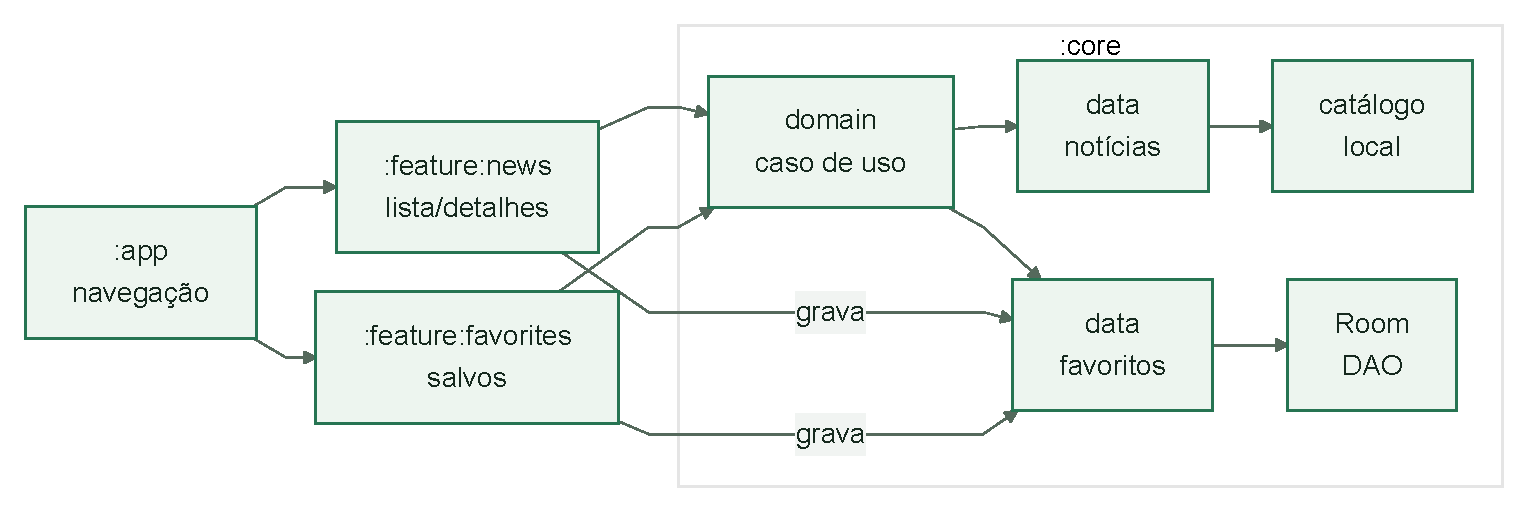
\includegraphics[width=\textwidth]{imagens/05-demo.pdf}
\caption{Arquitetura implementada na demonstração. Setas indicam dependências
ou chamadas; a atualização observável percorre o caminho inverso até a UI.}
\Description{O aplicativo coordena duas features. Ambas usam um caso de uso no núcleo e gravam pelo repositório de favoritos. O domínio combina catálogo local e favoritos Room.}
\label{fig:demo}
\end{figure*}

A validação aprovou \UnitTests{} testes unitários e \InstrumentedTests{}
instrumentados: caso de uso, repositórios, três ViewModels, Room real,
reabertura de arquivo e navegação Compose. O roteiro no emulador também
confirmou o favorito após encerrar e reabrir o processo. O lint não apontou
erros; avisos sobre versões mais novas foram preservados, pois as versões
foram fixadas por compatibilidade.

As verificações encontraram zero ciclos, zero dependências entre features e
zero referências proibidas à persistência no recorte da UI. Cinco classes
foram testadas com fakes; a chamada unitária levou \UnitSeconds{} s, com
cache e daemon ativos. Os cinco controles amostrados atenderam às verificações
de rótulo e área mínima de 48 dp.

No APK debug, em emulador Android 16 ARM64, dez reinícios do processo
apresentaram mediana de \StartupMedian{} ms
(intervalo \StartupMin{}--\StartupMax{} ms) para \texttt{Total\allowbreak Time}.
Dez gravações com Room em memória tiveram latência mediana de \FavoriteMedian{}
ms até a emissão combinada. Uma amostra após o roteiro registrou
\MemoryPss{} MiB de PSS. Essas observações não medem desempenho do NiA,
latência final de renderização ou comportamento em aparelhos físicos.

\section{Discussão}\label{sec:discussao}
A demonstração evidencia separação entre interação, composição de dados e
persistência. Repositórios e injeção permitiram controlar falhas nos testes;
isso não demonstra redução futura de defeitos. A presença de ViewModels
também não impede acúmulo de responsabilidades. O colaborador de estado evita
repetição, ao custo de mais uma abstração de apresentação.

Quatro módulos preservam isolamento de funcionalidades com menos configuração
que o original. Em contrapartida, as camadas dentro do núcleo têm limites de
pacotes, mais fracos que módulos de compilação independentes. A escolha atende
ao escopo acadêmico, sem pretender substituir a modularização do NiA.

Os resultados são exploratórios e descrevem um emulador em uma máquina,
com APK debug, cache de disco preservado e poucas amostras. Não houve comparação controlada de
arquiteturas nem estudo com usuários. Rótulos e áreas de toque verificáveis
não comprovam usabilidade global. As hipóteses sobre stakeholders também
precisariam de validação com participantes reais.

\section{Conclusão e Trabalhos Futuros}\label{sec:conclusao}
A inspeção identificou camadas, apresentação baseada em ViewModel, UDF,
repositórios, composição reativa, modularização, Hilt e persistência com
sincronização. O confronto entre documentação e código evitou reproduzir um
participante desatualizado no fluxo For You.

A aplicação independente concretizou um subconjunto dessas decisões e
permitiu testar navegação, atualização reativa e persistência de favoritos.
Stakeholders e GQM ajudaram a formular critérios explícitos, separando
observações de propostas. Como continuidade, propõem-se tarefas com usuários,
medições em dispositivos físicos e, apenas se o escopo exigir, uma fonte
remota com política de sincronização e migrações de banco.


\section*{Declaração de Uso de Inteligência Artificial}
O Codex auxiliou a inspeção documental, a redação, a implementação, os testes
e a preparação de diagramas e apresentação. As evidências de execução foram
registradas. A revisão e a responsabilidade acadêmica pelo material cabem aos
autores, que devem conferi-lo antes da submissão.

\bibliographystyle{ACM-Reference-Format}
\bibliography{referencias}
\end{document}
